\documentclass[11pt,conference,letterpaper]{IEEEtran}
\usepackage{amsmath,graphicx,booktabs}
\usepackage[hidelinks]{hyperref}
\newcommand{\F}{\ensuremath{F_1}}
\title{Distinguishing Single-Phase Earth Faults from Routine Switching in Power-Grid Recordings}
\author{\IEEEauthorblockN{Md. Aslam Hossain}\IEEEauthorblockA{Department of Electrical and Computer Engineering\\The University of Alabama in Huntsville, Huntsville, Alabama, USA\\mh0708@uah.edu}}
\begin{document}
\maketitle
\begin{abstract}
Can one electrical cycle distinguish a single-phase earth fault from routine switching in a recording unseen during training? I investigated this question using OscGrid field measurements. I first reproduced the published four-class multilayer perceptron benchmark. Across five runs, mean fault-event \F{} was 0.609 compared with the published 0.790, while no-event \F{} was 0.846 compared with 0.840. I then compared logistic regression and random forests on 2,416 labeled cycles from 86 recordings. A forest using five root-mean-square measurements achieved mean earth-fault \F{} of 0.946 across five fits on a recording-disjoint holdout (95\% recording-bootstrap interval 0.889--1.000). Adding two phase-spread features increased mean logistic-regression \F{} from 0.827 to 0.937 and decreased forest \F{} to 0.931. Both paired intervals for the change included zero. Six held-out recordings contained earth faults, limiting the precision of the comparison.
\end{abstract}
\begin{IEEEkeywords}power-system protection, relay oscillography, single-phase earth faults, random forest, logistic regression\end{IEEEkeywords}
\section{Introduction}
A protection engineer reviewing a disturbance faces a practical question. Did the waveform change because equipment switched as expected, or does the affected circuit warrant investigation for a fault? Both events can produce an abrupt change in voltage and current. A flag attached to a short interval could help the engineer locate a waveform that deserves closer inspection. Missed faults and unnecessary flags both matter for this use case.

OscGrid contains measurements from operating electrical networks and includes expert annotations \cite{osc,data}. Its published classification benchmark groups waveform behavior into four broad categories. A classifier that recognizes abnormal behavior has answered one useful question. An engineer looking specifically for single-phase earth faults needs a finer distinction within the annotations. A single disturbance recording can support both questions when the target is defined explicitly.

I conducted two experiments. The first examines how closely the published MLP scores can be reproduced from the released measurements and training implementation. The second asks whether simple features of one cycle can identify an earth fault in a held-out recording. I compared a linear classifier and an ensemble of decision trees. I also tested whether supplying the differences between phases explicitly helps either model. All three methods can be trained on a conventional computer.

\section{Problem Statement}
One binary example consists of a complete electrical cycle measured at one bus. The positive label indicates an expert-annotated single-phase earth fault. The negative label indicates routine switching. The classifier receives only analog features. Event annotations establish the reference labels and determine which cycles are eligible. When the classifier is evaluated, all buses and cycles from a test recording have been withheld together.

This definition bounds the engineering claim. The negative class excludes undisturbed operation, other abnormalities and critical short circuits. The experiment starts from annotated intervals and evaluates discrimination within them. Fault-onset delay, false alarms per day and the performance of a relay trip decision would require a continuous test stream, an alarm rule and suitable reference timings. The intended use here is retrospective waveform review.

I measured the fraction of labeled faults detected, the fraction of fault flags that were correct, and the change when two phase-spread features were added. I used the same test recordings for the two classifiers and both feature sets. This controls for the possibility that a representation appears easier simply because fewer difficult records qualify for it.

\section{Dataset}
\subsection{Source and event labels}
I used version 6 of OscGrid, released by its creators on Figshare \cite{data}. It comprises 50,765 oscillograms, with 480 expert-annotated recordings forming the starting pool. Relay protection and automation terminals on operating power grids supplied the original measurements. The researchers assembled the recordings from industrial databases and collaborating organizations, anonymized them, and released the data and processing code \cite{osc,code}. The labeled CSV contains sample indices, recording and bus identifiers, analog channels and annotation flags. Channel availability varies across records.

The published benchmark distinguishes no event, operational switching, abnormal events and fault events. The last group includes disturbances such as short circuits. For the binary task I selected the specific abnormal-event branch \texttt{ML\_2\_1}, including its earth-fault subtypes. Routine switching came from \texttt{ML\_1}. Thus a positive binary example can belong to the abnormal-event class in the benchmark. The two experiments require separate comparisons.

\subsection{Constructing a complete cycle}
All 480 labeled COMTRADE configuration files specified a nominal grid frequency of 50 Hz and sampling frequency of 1,600 Hz, giving 32 samples per nominal cycle. I formed nonoverlapping cycles aligned to multiples of 32 in the sample index. Each accepted interval contained all 32 distinct consecutive indices within the same recording, bus and event segment. Missing required measurements, discontinuities and label changes excluded a window.

Every sample in a positive cycle carried the earth-fault annotation or a subtype. I excluded simultaneous switching, critical faults and other specific abnormal-event branches. Each negative cycle carried a switching annotation throughout without a concurrent abnormal or fault event. A recording could contribute a fault during one interval and switching later. Keeping both intervals under the same recording identifier was essential to the split.

\subsection{Eligibility and the proposal change}
My proposal specified three phase currents and three busbar phase voltages. Requiring all six measured quantities left eight positive cycles, all from a single recording (Table~\ref{tab:audit}). That would force a choice between training on that positive recording and independently testing on it. The source configuration files for 22 of the 23 otherwise eligible fault recordings listed phase-A and phase-C currents without a phase-B current channel. Filling those entries with zero would encode an unsupported physical value.
\begin{table}[t]\centering\caption{Usable recordings and nonoverlapping cycles. A recording can contribute both labels at different times.}\label{tab:audit}
\begin{tabular}{llrr}\toprule Signals & Class & Recordings & Cycles\\\midrule
Six & Switching &35&842\\ Six & Earth fault &1&8\\
Five & Switching &83&1,572\\ Five & Earth fault &23&844\\\bottomrule\end{tabular}\end{table}

I retained currents on phases A and C and busbar voltages on all three phases. This yielded 86 distinct recordings: 63 provided only switching, three provided only faults, and 20 provided both. The 844 positive and 1,572 negative cycles account for 77,312 bus-level sample rows. Several buses from a disturbance can supply examples. The number of independent fault recordings remains a more useful guide to the strength of the evaluation than the number of rows alone.

\section{Methods}
\subsection{Reproduction of the four-class MLP}
I followed the released supervised training implementation \cite{code}. Its inputs were the same five analog channels, but the MLP retained the individual waveform samples. I removed rows missing a required input and assigned the benchmark class in descending order of annotation priority: fault events, abnormal events, then switching. Rows with no active event flag received class zero. A change in file identifier or target started a new block. Blocks shorter than 32 samples were discarded.

Blocks were shuffled and assigned within each class, targeting 60\% training, 10\% validation and 30\% testing by sample count. A frame spanned 32 samples at stride ten within one block. The class remained constant throughout the frame, so its label agreed with the center-weighted vote in the released implementation. I standardized the channels using training samples and flattened each frame into 160 inputs. The MLP had a 128-unit hidden layer, batch normalization, ReLU activation, dropout of 0.3 and four output logits.

Training used inverse-frequency weighted cross-entropy, batch size 128, learning rate 0.001 and gradient clipping at norm ten. I followed the released code's AdamW optimizer with weight decay 0.0001. The article describes Adam \cite{osc,code}. I restored the best validation-accuracy checkpoint, with patience ten and a maximum of 100 epochs. Seed 443 came from the released script, and I selected 444--447 for the remaining runs. The seed changes block assignment and training randomness together. Batching precomputed windows can produce a different minibatch order from the authors' data loader.

\subsection{Binary feature processing}
For measured signal $x$ within an eligible cycle, I computed the root mean square (RMS) over 32 samples,
\begin{equation} r(x)=\sqrt{\frac{1}{32}\sum_{j=0}^{31}x_j^2}. \end{equation}
The baseline vector comprised $r(I_A),r(I_C),r(V_A),r(V_B),r(V_C)$ on the released CSV scale. RMS retains information about magnitude and discards phase angle and sample order. I used busbar voltages consistently so that switching measurement location would not change the definition of an input.

For the expanded representation, I appended
\begin{align}
d_I &= |r(I_A)-r(I_C)|,\\
d_V &= \max_{p\in\{A,B,C\}}r(V_p)-\min_{p\in\{A,B,C\}}r(V_p).
\end{align}
The current term compares two measured phases; the voltage term spans three phases. Both are deterministic functions of the original inputs. They can still affect performance by changing the decision boundaries a particular classifier can represent. For example, a large current difference can arise when either phase has the larger RMS. A coefficient on $d_I$ can respond in the same direction in both cases.

\subsection{Models and parameter tuning}
For standardized inputs $z$, logistic regression estimates fault probability using an intercept $b$ and weight vector $w$:
\begin{equation}
\widehat p(y=1\mid z)=\left(1+\exp[-(b+w^{\mathsf T}z)]\right)^{-1}.
\end{equation}
I fitted the model using L2 regularization \cite{isl}. Scaling parameters were estimated inside each training fold. The alternative was a random forest of 120 trees \cite{forest}. A forest averages the estimated class probabilities from its trees. Threshold splits on current and voltage can represent interactions among the channels. For either model, a cycle was flagged when its estimated probability reached the selected threshold.

With seed 443, I assigned 64 recordings to development and 22 to the final holdout. Stratification used the presence of at least one eligible fault cycle in a recording. The development partition contained 583 fault and 1,192 switching cycles. The holdout contained 261 fault and 380 switching cycles. Seventeen development recordings and six test recordings supplied positive cycles. All 22 test recordings supplied switching cycles.

Within development data I used four stratified folds of recording identifiers. The logistic-regression inverse penalty strengths were $C\in\{0.1,1,10\}$. Forest depth candidates were three, six and unrestricted. I pooled out-of-fold probabilities for each candidate and evaluated thresholds 0.3 through 0.7 in steps of 0.1. The parameter and threshold maximizing validation fault \F{} were retained, and the model was fitted on all development recordings. Each feature set was tuned separately. Consequently, its ablation effect includes differences in the selected operating point.

\subsection{Evaluation and uncertainty}
Let $T$, $P$ and $N$ denote true positives, false positives and false negatives. Fault precision is $T/(T+P)$, recall is $T/(T+N)$ and
\begin{equation}F_1=\frac{2T}{2T+P+N}.\end{equation}
I scored individual cycles, giving longer eligible intervals greater influence on the score. For the binary experiment I repeated the final fits using seeds 443--447. The split, tuned settings and thresholds remained fixed. Only the random forest introduces stochastic variation in this setup. In the MLP experiment, a different seed also changes the split.

For the binary scores I drew 5,000 bootstrap samples of held-out recordings, with replacement within the two fault-presence strata. Every cycle from a sampled recording traveled together. I used identical draws across model seeds and feature sets. For each draw I computed cycle-level \F{} and averaged across seeds. The 2.5th and 97.5th percentiles give the reported limits. For the paired comparison I took the difference $F_{1,7}-F_{1,5}$ on each draw before computing the percentiles. These intervals quantify variation in which test recordings are represented, conditional on the original development set and fitted models.
\section{Results}
\subsection{Four-class benchmark reproduction}
Table~\ref{tab:mlp} compares the five-run means. The no-event scores differed by 0.006. Operational switching had the lowest published MLP score and improved by 0.051 in the reproduction. The reproduced abnormal-event score fell by 0.031. The largest difference was a reduction of 0.181 for fault events. Overall accuracy alone would conceal that class-specific discrepancy.
\begin{table}[t]\centering\caption{Mean MLP test \F{}. Published values are from Table 2 of Evdakov et al.~\cite{osc}.}\label{tab:mlp}
\begin{tabular}{lrrr}\toprule Class & Published & Reproduced & Change\\\midrule
No event&0.840&0.846&$+$0.006\\
Operational switching&0.450&0.501&$+$0.051\\
Abnormal events&0.810&0.779&$-$0.031\\
Fault events&0.790&0.609&$-$0.181\\\bottomrule\end{tabular}\end{table}

Fault-event scores at seeds 443--447 were 0.696, 0.051, 0.857, 0.747 and 0.694. At seed 444, fault precision was 0.066 and recall was 0.042. That run missed most labeled fault windows, and most predicted fault windows were incorrect. Seed 445 had the highest fault score. Since both test composition and training randomness changed, these runs cannot isolate the cause of the variation.

At seed 443, the released protocol yielded 69,366 training, 11,447 validation and 34,691 test frames. Of 283 test recording identifiers, 229 also occurred in training through different blocks. The block partition preserves comparability with the released benchmark. The binary evaluation addresses a separate generalization question by withholding whole recordings. Its positives refer to a different annotation level. A larger numerical binary score therefore cannot establish an improvement over the published four-class model.

\subsection{Earth-fault classification}
Table~\ref{tab:fit} gives the selected parameters and the test scores at seed 443. With five RMS features the forest selected a maximum depth of three and a threshold of 0.5. It detected 245 of 261 fault cycles and classified 369 of 380 switching cycles correctly (Fig.~\ref{fig:cm}). This corresponds to a 6.1\% missed-fault fraction and a 2.9\% false-positive fraction among switching cycles.
\begin{table}[t]\centering\caption{Held-out cycle scores at seed 443. LR denotes logistic regression and RF denotes random forest.}\label{tab:fit}
\setlength{\tabcolsep}{3.3pt}\begin{tabular}{llrrrr}\toprule Model & Setting & Threshold & Precision & Recall & $F_1$\\\midrule
LR, 5 & $C=10$ & .6 &1.000&.705&.827\\
LR, 7 & $C=10$ & .3 &1.000&.881&.937\\
RF, 5 & depth 3 & .5 &.957&.939&.948\\
RF, 7 & depth 6 & .7 &1.000&.862&.926\\\bottomrule\end{tabular}\end{table}
\begin{figure}[t]\centering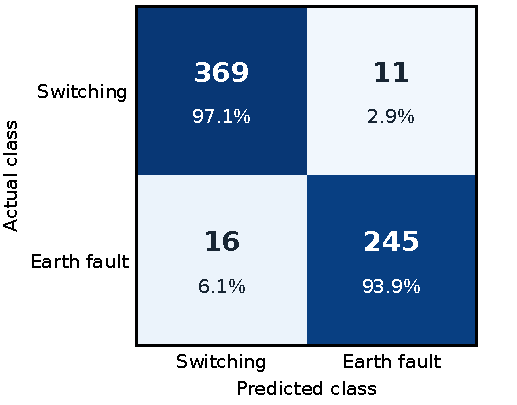
\includegraphics[width=.94\columnwidth]{forest5_confusion_matrix.pdf}
\caption{Held-out decisions for the five-feature forest at seed 443. Counts are individual cycles. Percentages use each true class total.}\label{fig:cm}\end{figure}

The seven-feature logistic model raised zero false alarms on the same holdout and missed 31 fault cycles. The five-feature forest recovered 15 more fault cycles at the cost of 11 switching alerts. An engineer prioritizing sensitivity might accept those additional alerts, whereas a reviewer with limited time might place greater weight on precision. Validation \F{} determined the operating points here; no specific cost ratio for missed faults and false alarms was assumed.

Errors clustered within recordings. All 11 false alarms from the five-feature forest came from one recording. Thirteen of its 16 missed fault cycles came from one recording and the other three came from a second. Eleven flagged cycles therefore need not represent eleven separate incidents. Figure~\ref{fig:waves} traces one false alarm and one missed fault to their original waveforms. Each curve has 32 measured values, which the classifier reduces to a single RMS value. Phase displacement and within-cycle waveform shape are examples of information lost in this reduction. The plots illustrate this limitation but do not establish the cause of either error.

\begin{figure*}[t]\centering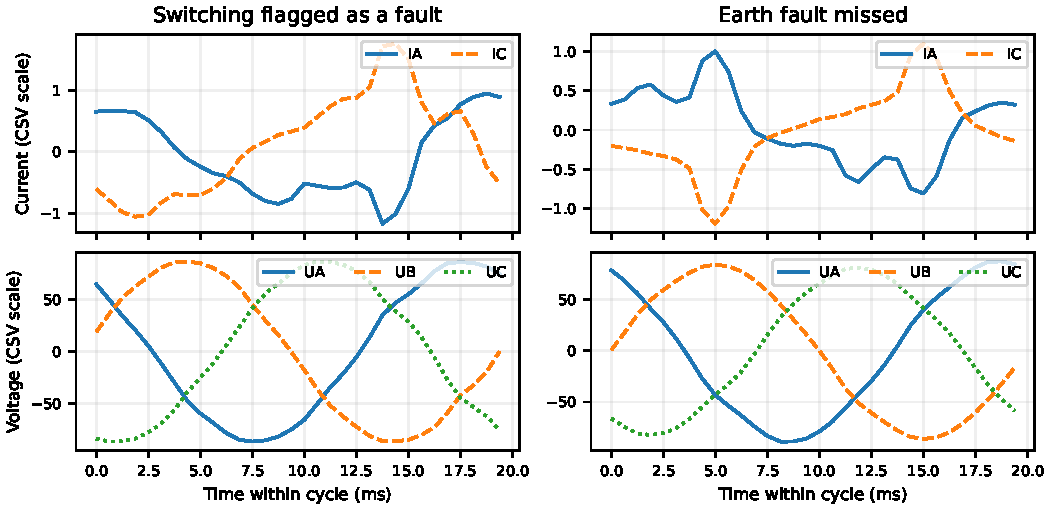
\includegraphics[width=.90\textwidth]{error_cycles.pdf}
\caption{Misclassified holdout cycles for the five-feature forest. The switching cycle flagged as a fault begins at sample 2176 on bus 2 of recording cc91716e (left). The missed fault begins at sample 6496 on bus 1 of recording 524e846b (right). For each error type I plotted the first example sorted by recording, bus and sample. IDs are abbreviated; vertical scales are local to each panel.}\label{fig:waves}\end{figure*}

\subsection{Feature ablation across repeated fits}
Across five fits, the five-feature forest gave mean fault \F{} of 0.946 (range 0.944--0.948). With seven features the mean was 0.931 (range 0.926--0.939). Logistic regression produced identical scores across the repeated fits, with the mean rising from 0.827 to 0.937 when both spread features were added. For the five-feature forest, the 95\% recording-level interval was 0.889--1.000. Its width compared with the narrow across-seed range illustrates that repeatability of training and uncertainty in the test population measure different things.
\begin{figure*}[t]\centering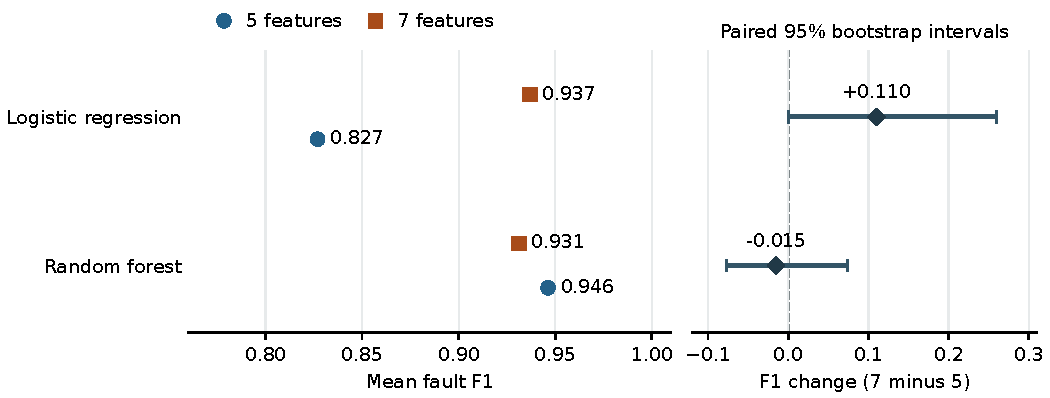
\includegraphics[width=.90\textwidth]{feature_comparison.pdf}
\caption{Mean fault \F{} across five fits on the common holdout (left) and paired recording-bootstrap intervals for the change after adding two spread features (right). Zero represents equal mean \F{}.}\label{fig:ab}\end{figure*}

The logistic-regression change was $+0.110$ (paired 95\% interval 0.000 to 0.260). The forest change was $-0.015$ ($-0.077$ to 0.073), as shown in Fig.~\ref{fig:ab}. The linear model's point estimate is consistent with a benefit from explicitly encoding imbalance, but its interval reaches zero. The forest interval spans both directions. The results support reporting the observed ordering on this split while leaving open whether either feature change would be reliable across new disturbances.

\subsection{Data and Code Availability}
I used \texttt{labeled.csv} from the \texttt{labeled.7z} archive in \href{https://doi.org/10.6084/m9.figshare.28465427.v6}{OscGrid version 6 on Figshare} \cite{data}. The release also provides raw COMTRADE files and channel and annotation dictionaries. The original data collection is documented in \cite{osc}. My training scripts, eligibility audits, split assignments, predictions, seed-level scores and comparison figures are available in the \href{https://github.com/tornadochilddgh/tornadochildd/tree/a505abcb0a3388b1732c2d8e828513bec3bfed54}{project repository at experiment commit a505abcb} \cite{mine}. The file \texttt{predictions.csv} identifies the recording, bus and first sample of each held-out cycle, allowing an individual error to be traced to its waveform.

\section{Discussion and Limitations}
The eligibility audit changed which engineering question could be tested independently. Requiring all three phase currents would have left one recording to supply every positive example. Using five measured channels retained 23 positive recordings without imputing a missing waveform. The results apply to the specified pair of currents and the three busbar voltages. The current difference should not be interpreted as a full three-phase current-imbalance measurement.

The test set contained 261 positive cycles out of 641 eligible cycles. Precision depends on that proportion, which arose from the expert annotations and eligibility rules. An operator scanning an entire archive might encounter a different mix. In addition, one of the six fault-bearing holdout recordings contributed 97 positive cycles. The response to one long event can therefore have a substantial influence on cycle-level recall. A follow-up evaluation could define an alarm using successive flags and count false alarm episodes and time to first detection.

Holding the split fixed isolates forest training variability and supports a paired feature comparison. Different development recordings, acquisition systems or sites might produce different tuned settings. More independently annotated faults would allow those changes to be examined. The six fault-bearing test recordings limit the strength of claims about generalization even though each recording contains many waveform samples.

\section{Conclusion}
I repeated the published four-class MLP experiment using five random seeds. For the no-event class, my mean F1 score of 0.846 closely matched the published value of 0.840. For the fault-event class, my mean F1 score was 0.609, well below the published value of 0.790.For the separate task of distinguishing single-phase earth faults from routine switching, I compared logistic regression and a shallow random forest on the same 22 held-out recordings. The forest achieved the highest observed mean fault F1 score of 0.946 using five RMS features calculated over one electrical cycle. Adding two features that measured differences between phases raised the logistic regression score from 0.827 to 0.937 and lowered the forest score from 0.946 to 0.931. For both models, the paired 95\% bootstrap interval for the change in F1 included zero, leaving the effect of the added features uncertain.

These results suggest that one cycle of current and voltage measurements can help a protection engineer distinguish earth faults from routine switching when reviewing a recorded disturbance. Only six held-out recordings contained an earth fault, and the classification errors were concentrated in a few recordings. Testing the classifier on additional independent fault recordings is the next step in assessing how well it generalizes.

\begin{thebibliography}{6}
\bibitem{osc} A. Evdakov, G. Filatova, A. Yablokov, A. Kovalenko, E. Skachkov, and I. Makarov, A dataset of real-world oscillograms from electrical power grids, \emph{Scientific Data}, vol. 13, art. 262, 2026. \href{https://doi.org/10.1038/s41597-026-06587-8}{doi: 10.1038/s41597-026-06587-8}.
\bibitem{data} A. Evdakov, A. Makoldin, A. Kovalenko, G. Filatova, and A. Yablokov, \emph{A Dataset of Real-World Oscillograms from Electric Power Grids}, Figshare, ver. 6, 2025. \href{https://doi.org/10.6084/m9.figshare.28465427.v6}{doi: 10.6084/m9.figshare.28465427.v6}.
\bibitem{code} AIRI Institute, OscGrid source code, revision \texttt{4cbdf81}. \url{https://github.com/AIRI-Institute/oscgrid}
\bibitem{isl} G. James, D. Witten, T. Hastie, R. Tibshirani, and J. Taylor, \emph{An Introduction to Statistical Learning: With Applications in Python}. Springer, 2023.
\bibitem{forest} L. Breiman, Random forests, \emph{Machine Learning}, vol. 45, pp. 5--32, 2001. \href{https://doi.org/10.1023/A:1010933404324}{doi: 10.1023/A:1010933404324}.
\bibitem{mine} M. A. Hossain, OscGrid benchmark reproduction and earth-fault classification, GitHub, experiment commit \texttt{a505abcb}. \url{https://github.com/tornadochilddgh/tornadochildd}
\end{thebibliography}
\end{document}
